%%
%% This is file `sample-manuscript.tex',
%% generated with the docstrip utility.
%%
%% The original source files were:
%%
%% samples.dtx  (with options: `manuscript')
%% 
%% IMPORTANT NOTICE:
%% 
%% For the copyright see the source file.
%% 
%% Any modified versions of this file must be renamed
%% with new filenames distinct from sample-manuscript.tex.
%% 
%% For distribution of the original source see the terms
%% for copying and modification in the file samples.dtx.
%% 
%% This generated file may be distributed as long as the
%% original source files, as listed above, are part of the
%% same distribution. (The sources need not necessarily be
%% in the same archive or directory.)
%%
%% Commands for TeXCount
%TC:macro \cite [option:text,text]
%TC:macro \citep [option:text,text]
%TC:macro \citet [option:text,text]
%TC:envir table 0 1
%TC:envir table* 0 1
%TC:envir tabular [ignore] word
%TC:envir displaymath 0 word
%TC:envir math 0 word
%TC:envir comment 0 0
%%
%%
%% The first command in your LaTeX source must be the \documentclass command.
%%%% Small single column format, used for CIE, CSUR, DTRAP, JACM, JDIQ, JEA, JERIC, JETC, PACMCGIT, TAAS, TACCESS, TACO, TALG, TALLIP (formerly TALIP), TCPS, TDSCI, TEAC, TECS, TELO, THRI, TIIS, TIOT, TISSEC, TIST, TKDD, TMIS, TOCE, TOCHI, TOCL, TOCS, TOCT, TODAES, TODS, TOIS, TOIT, TOMACS, TOMM (formerly TOMCCAP), TOMPECS, TOMS, TOPC, TOPLAS, TOPS, TOS, TOSEM, TOSN, TQC, TRETS, TSAS, TSC, TSLP, TWEB.
% \documentclass[acmsmall]{acmart}

%%%% Large single column format, used for IMWUT, JOCCH, PACMPL, POMACS, TAP, PACMHCI
% \documentclass[acmlarge,screen]{acmart}

%%%% Large double column format, used for TOG
% \documentclass[acmtog, authorversion]{acmart}

%%%% Generic manuscript mode, required for submission
%%%% and peer review
\documentclass[sigconf,authordraft,acmsmall]{acmart}
%% Fonts used in the template cannot be substituted; margin 
%% adjustments are not allowed.
%%
%% \BibTeX command to typeset BibTeX logo in the docs
\AtBeginDocument{%
  \providecommand\BibTeX{{%
    \normalfontB\kern-0.5em{\scshape i\kern-0.25em b}\kern-0.8em\TeX}}}

%% Rights management information.  This information is sent to you
%% when you complete the rights form.  These commands have SAMPLE
%% values in them; it is your responsibility as an author to replace
%% the commands and values with those provided to you when you
%% complete the rights form.
\setcopyright{acmcopyright}
\copyrightyear{2018}
\acmYear{2018}
\acmDOI{XXXXXXX.XXXXXXX}

%% These commands are for a PROCEEDINGS abstract or paper.
% \acmConference[Conference acronym `XX]{Make sure to enter the correct
%   conference title from your rights confirmation emai}{June 03--05,
%   2018}{Woodstock, NY}
%
%  Uncomment \acmBooktitle if th title of the proceedings is different
%  from ``Proceedings of ...''!
%
% \acmBooktitle{Woodstock '18: ACM Symposium on Neural Gaze Detection,
%  June 03--05, 2018, Woodstock, NY} 
% \acmPrice{15.00}
% \acmISBN{978-1-4503-XXXX-X/18/06}


%%
%% Submission ID.
%% Use this when submitting an article to a sponsored event. You'll
%% receive a unique submission ID from the organizers
%% of the event, and this ID should be used as the parameter to this command.
%%\acmSubmissionID{123-A56-BU3}

%%
%% For managing citations, it is recommended to use bibliography
%% files in BibTeX format.
%%
%% You can then either use BibTeX with the ACM-Reference-Format style,
%% or BibLaTeX with the acmnumeric or acmauthoryear sytles, that include
%% support for advanced citation of software artefact from the
%% biblatex-software package, also separately available on CTAN.
%%
%% Look at the sample-*-biblatex.tex files for templates showcasing
%% the biblatex styles.
%%

%%
%% The majority of ACM publications use numbered citations and
%% references.  The command \citestyle{authoryear} switches to the
%% "author year" style.
%%
%% If you are preparing content for an event
%% sponsored by ACM SIGGRAPH, you must use the "author year" style of
%% citations and references.
%% Uncommenting
%% the next command will enable that style.
%%\citestyle{acmauthoryear}
% \input{macros/preamble}
% \input{macros/math}
%%
%% end of the preamble, start of the body of the document source.
\usepackage{subcaption} 

\theoremstyle{definition}
\newtheorem{exmp}{Example}

\begin{document}

%%
%% The "title" command has an optional parameter,
%% allowing the author to define a "short title" to be used in page headers.
\title{Challenges in Impleneting client side compilation using WebAssembly}

%%
%% The "author" command and its associated commands are used to define
%% the authors and their affiliations.
%% Of note is the shared affiliation of the first two authors, and the
%% "authornote" and "authornotemark" commands
%% used to denote shared contribution to the research.
\author{VJS Pranavasri}
\email{vjs.pranavasri@research.iiit.ac.in}
\affiliation{%
  \institution{International Institute of Information Technology}
  \streetaddress{Professor CR Rao Road, Gachibowli}
  \city{Hyderabad}
  \state{Telangana}
  \country{India}
  \postcode{500032}
}

% \author{Lars Th{\o}rv{\"a}ld}
% \affiliation{%
%   \institution{The Th{\o}rv{\"a}ld Group}
%   \streetaddress{1 Th{\o}rv{\"a}ld Circle}
%   \city{Hekla}
%   \country{Iceland}}
% \email{larst@affiliation.org}

% \author{Valerie B\'eranger}
% \affiliation{%
%   \institution{Inria Paris-Rocquencourt}
%   \city{Rocquencourt}
%   \country{France}
% }

% \author{Aparna Patel}
% \affiliation{%
%  \institution{Rajiv Gandhi University}
%  \streetaddress{Rono-Hills}
%  \city{Doimukh}
%  \state{Arunachal Pradesh}
%  \country{India}}

% \author{Huifen Chan}
% \affiliation{%
%   \institution{Tsinghua University}
%   \streetaddress{30 Shuangqing Rd}
%   \city{Haidian Qu}
%   \state{Beijing Shi}
%   \country{China}}

% \author{Charles Palmer}
% \affiliation{%
%   \institution{Palmer Research Laboratories}
%   \streetaddress{8600 Datapoint Drive}
%   \city{San Antonio}
%   \state{Texas}
%   \country{USA}
%   \postcode{78229}}
% \email{cpalmer@prl.com}

% \author{John Smith}
% \affiliation{%
%   \institution{The Th{\o}rv{\"a}ld Group}
%   \streetaddress{1 Th{\o}rv{\"a}ld Circle}
%   \city{Hekla}
%   \country{Iceland}}
% \email{jsmith@affiliation.org}

% \author{Julius P. Kumquat}
% \affiliation{%
%   \institution{The Kumquat Consortium}
%   \city{New York}
%   \country{USA}}
% \email{jpkumquat@consortium.net}

%%
%% By default, the full list of authors will be used in the page
%% headers. Often, this list is too long, and will overlap
%% other information printed in the page headers. This command allows
%% the author to define a more concise list
%% of authors' names for this purpose.
% \renewcommand{\shortauthors}{Trovato and Tobin, et al.}

%%
%% The code below is generated by the tool at http://dl.acm.org/ccs.cfm.
%% Please copy and paste the code instead of the example below.
%%
\begin{CCSXML}
  <ccs2012>
     <concept>
         <concept_id>10011007.10011006.10011039.10011311</concept_id>
         <concept_desc>Software and its engineering~Semantics</concept_desc>
         <concept_significance>500</concept_significance>
         </concept>
     <concept>
         <concept_id>10011007.10010940.10010971.10010980.10010982</concept_id>
         <concept_desc>Software and its engineering</concept_desc>
         <concept_significance>300</concept_significance>
         </concept>
   </ccs2012>
\end{CCSXML}
  
\ccsdesc[500]{Software and its engineering~Semantics}
\ccsdesc[300]{Software and its engineering}

%%
%% Keywords. The author(s) should pick words that accurately describe
%% the work being presented. Separate the keywords with commas.
\keywords{WASM,Compilers,Software Engineering}


%%
%% The abstract is a short summary of the work to be presented in the
%% article.
\begin{abstract}
    WebAssembly compilers are tools that allow users to compile their code into the WebAssembly format. This format can be run on web browsers and other platforms that support the WebAssembly standard. We look at practical application of a webassembly compiler running on client side and study the challenges that arise in doing so. We present a prototype implementation of a webassembly compiler that runs on client side and discuss the challenges that we faced in implementing it. We also present a solution to the challenges that we faced.
\end{abstract}

% To create a state action pair
% The extra \ is to give a space
% $a \xto{{\sf myFunc}(params)}{Below Arrow_{subscript}} b$
% $a\ \xto{{\sf myFunc}(params)}{Below Arrow_{subscript}}\ b$

%%
%% This command processes the author and affiliation and title
%% information and builds the first part of the formatted document.
\maketitle

\section{Introduction}
WebAssembly (Wasm)\cite{wasm} is a web standard that defines a binary format and a corresponding assembly-like text format for executable code in web pages. The Wasm text format is designed as a portable, size-efficient, and embeddable format that runs with near-native performance and provides languages with low-level memory models such as C++ and Rust with a compilation target so that they can run on the web.
A webassembly compiler is a tool that converts a code written in a high-level language like C++ or Rust into webassembly code. This code can be run on a web browser or on a web server. \\
The main focus of this paper would be a study on such web compilers which themselves are written in webassembly. We first start with looking at the available solutions for the same. We then go on with pyodide as a base for our implementation. We then discuss the challenges that we faced in implementing a webassembly compiler on client side. We will broadly try to validate the study on WebAssembly compiler bugs\cite{bugsinwasm} \\
We will use Virtual Labs as a platform, where we test out our implementation for validaing our study. \\
We ask the following Research Questions to guide our study:
\begin{itemize}
    \item \textbf{RQ1:} How will the implementation of a webassembly compiler help in the development of web applications?
    \item \textbf{RQ2:} What are the challenges in implementing a webassembly compiler on client side?
    \item \textbf{RQ3:} How big of an impact do bugs in WebAssembly compilers have on the implementation requirement of Virtual Labs?
\end{itemize}
% Maybe consider making it the background section
\section{Virtual Labs}
Virtual Labs is an initiative by the Ministry of Human Resource Development (MHRD), Government of India, under the aegis of the National Mission on Education through Information and Communication Technology (NMEICT). This is coordinated by 12 participating institutes of which IIIT Hyderabad is a part. The main goal is to make any lab or education available independently of the platform. Virtual Labs mainly help professors and students who do not have proper lab facilities available by virtually emulating the scenario. \\
One of the current challenges faced by Virtual Labs is the ability to run code. This is mainly because of the requirement of a backend server to run the code. As the number of students using Virtual Labs increases, the load on the backend server increases. This is mainly because of the fact that the code will be run on the server and the results are sent back to the client. This would take a toll on the resources of the server. \\
The solution to this problem is to run the code on the client side. This would eliminate the need for a backend server, and possibly also allow interacting with the lab without any network after the first time. \\
For the scope of this paper, we would be working on a Python based Virtual Lab and we will be using pyodide as a base for our study and implementation. \\

\begin{figure}
    \centering
    \subcaptionbox{Server Side Compiling}
        {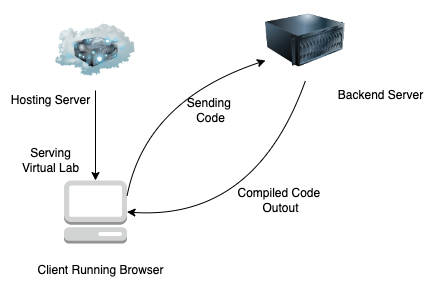
\includegraphics[width=0.55\textwidth]{images/server-model.png}}
    \subcaptionbox{Client Side Compiling}
        {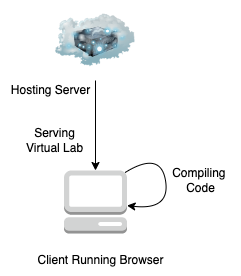
\includegraphics[width=0.35\textwidth]{images/client-model.png}}
    \caption{Server Side Model vs Client Side Model}
    \label{fig:csr vs ssr}
\end{figure}

\section{Related Work}
There is a lot of active study happening in the area of webassembly compilers, however we specifically focus on the ones that themseleves are written in webassembly that allows for client side compilations of other high/low level languages.

\subsection*{WebAssembly}
We take a lot of motivation from the paper that initially introduced webassembly to the world\cite{wasm}. The paper explains the gap in web devlopment which cannot inherenyly be solved by using javascript. This in depth describes major components WebAssembly as a language and a tool. One of the main goal being able to run cross language codes.

\subsection*{Study on WebAssembly}
With the introduction of the new byte code format, a lot of analysis in terms of performance and security has been done. The paper \cite{wasm-mech-verify} dicusses about the mechanisms of webassembly and how they verify the correctness of WASM. Then there ar multiple studies that go on to talk about performance of webassembly applications. \\
The paper \cite{wasm-perf-0} talks about how performance of web assembly based applications are and how different parameters like JIT(Just In Time) compilation and other factors affect the performance. Further studies focus on performance comparisions and energy consumption of webassembly applications compared to native applications\cite{wasm-perf-comp-0}. An intersting study was one that used WebAssembly to study the memory model of javascript and propose changes to improve consistency\cite{wasm-js-memory}. \\
A final research area is mainly geared towards security. The paper \textit{Everything Old is New Again}\cite{wasm-secur-0} talks about binary security of web assembly, as we are again now moving towards assembly format for the web. We see a paper that talks about the security in place for web assembly compilers\cite{wasmsecurity}. We would briefly refer to this to talk about security concerns that we find, and finally use the paper that does a performance analysis of webassembly compilers\cite{wasmtojs} as basis for our performance analysis.

\subsection*{WebAssembly Applications \& Compilers}
We look at some existing applications and compiler implementations to gain a better understanding. One such is an implementation of the e-commerce website ebay using WASM\cite{padmanabhan2020webassembly}. Then we look at an implementation of tensorflow backend which has been ported to web through WASM\cite{smilkov2020introducing}, this allows for running models on web through client. Before heading further we look at one of the most popular compilers that is written for C, emscripten\cite{zakai2011emscripten}. Emscripten is a compiler that compiles C/C++ to WASM. It is one of the most popular compilers for WASM.

\subsection*{Bugs in WebAssembly Compilers}
As we are focused more on the compilers that compile to WebAssembly, we use this paper as a base for our study\cite{bugsinwasm}. This paper discusses the bugs that are present in the WebAssembly compilers. We use this to compare and study its effects the implementation of Virtual Labs.

We see that there isn't that major of work being done in fields of web assembly compilers, and nothing specific to running them on client side. This would vouch for the novelty of the paper and we use the remotely similar work as a base for our study. For this paper we will be specifically focussing on pyodide, a python distribution that runs on browser\cite{pyodide}. We will be using this as a base for our study and implementation. The source code for the same is available on github.\footnote{\url{https://github.com/pyodide/pyodide}}

\section{Methodology}
Initially we do a collection of bugs from Pyodide repo. We then go ahead to analyse these bugs and try to compare them to the bugs proosed by Romano et al. \cite{bugsinwasm}. 

\subsection{Bugs Collection}
Our first goal is data collection. We follow the methods proposed followed by \cite{bugsinwasm} and use Github Search API\cite{githubsearchapi} and Github REST API\cite{githubrestapi} to collect all issues and pull requests. The project has a total of 880 Closed and 277 Open issues at the time of collection. For our use case, we filter out all the issues with label bug. This brings the total issues down tp 149 (closed) + 43 (open). We go through a detailed analysis of each issue and seggregate them based on the categories as shown in table \ref{tab:categories_bugs}. For the scope of the research course, we look at only the closed issues and filter out all duplicate bugs, won't-fix bugs and any bugs in the build time of pyodide. We majorly look at issues that are posed which are more focused with respect to pyodide as a framework itself or one of it's dependency CPython, emscripten or WebAssembly amongst others\footnote{The complete list of bugs is avaialble on sheets \url{https://stagbin.tk/pyodide_issues}}.

\begin{table}[]
    \begin{tabular}{|l|l|}
        \hline
        \textbf{Category}               & \textbf{Number of Unique Issues}  \\ \hline
        Asyncify Synchronous Code       &           1                       \\ \hline
        Incompatible Data Type          &           3                       \\ \hline
        Memory Model Differences        &           7                       \\ \hline
        Other Infrastructure Bug        &           12                      \\ \hline
        Emulating Native Environment    &           1                       \\ \hline
        Supporting Web API's            &           6                       \\ \hline
        Pyodide Specific                &           21                      \\ \hline
    \end{tabular}
\caption{Categories of issues taken from \cite{bugsinwasm}}
\label{tab:categories_bugs}
\end{table}

\subsection{Analysis}

\section{Implementation}
The main goal for realising client side compilation is to extend the existing virtual labs to add support to work as an online coding platform. The current implementation which can be used to compile and run code written in different languages, starting with python using pyodide.
\begin{figure}[h]
    \centering
    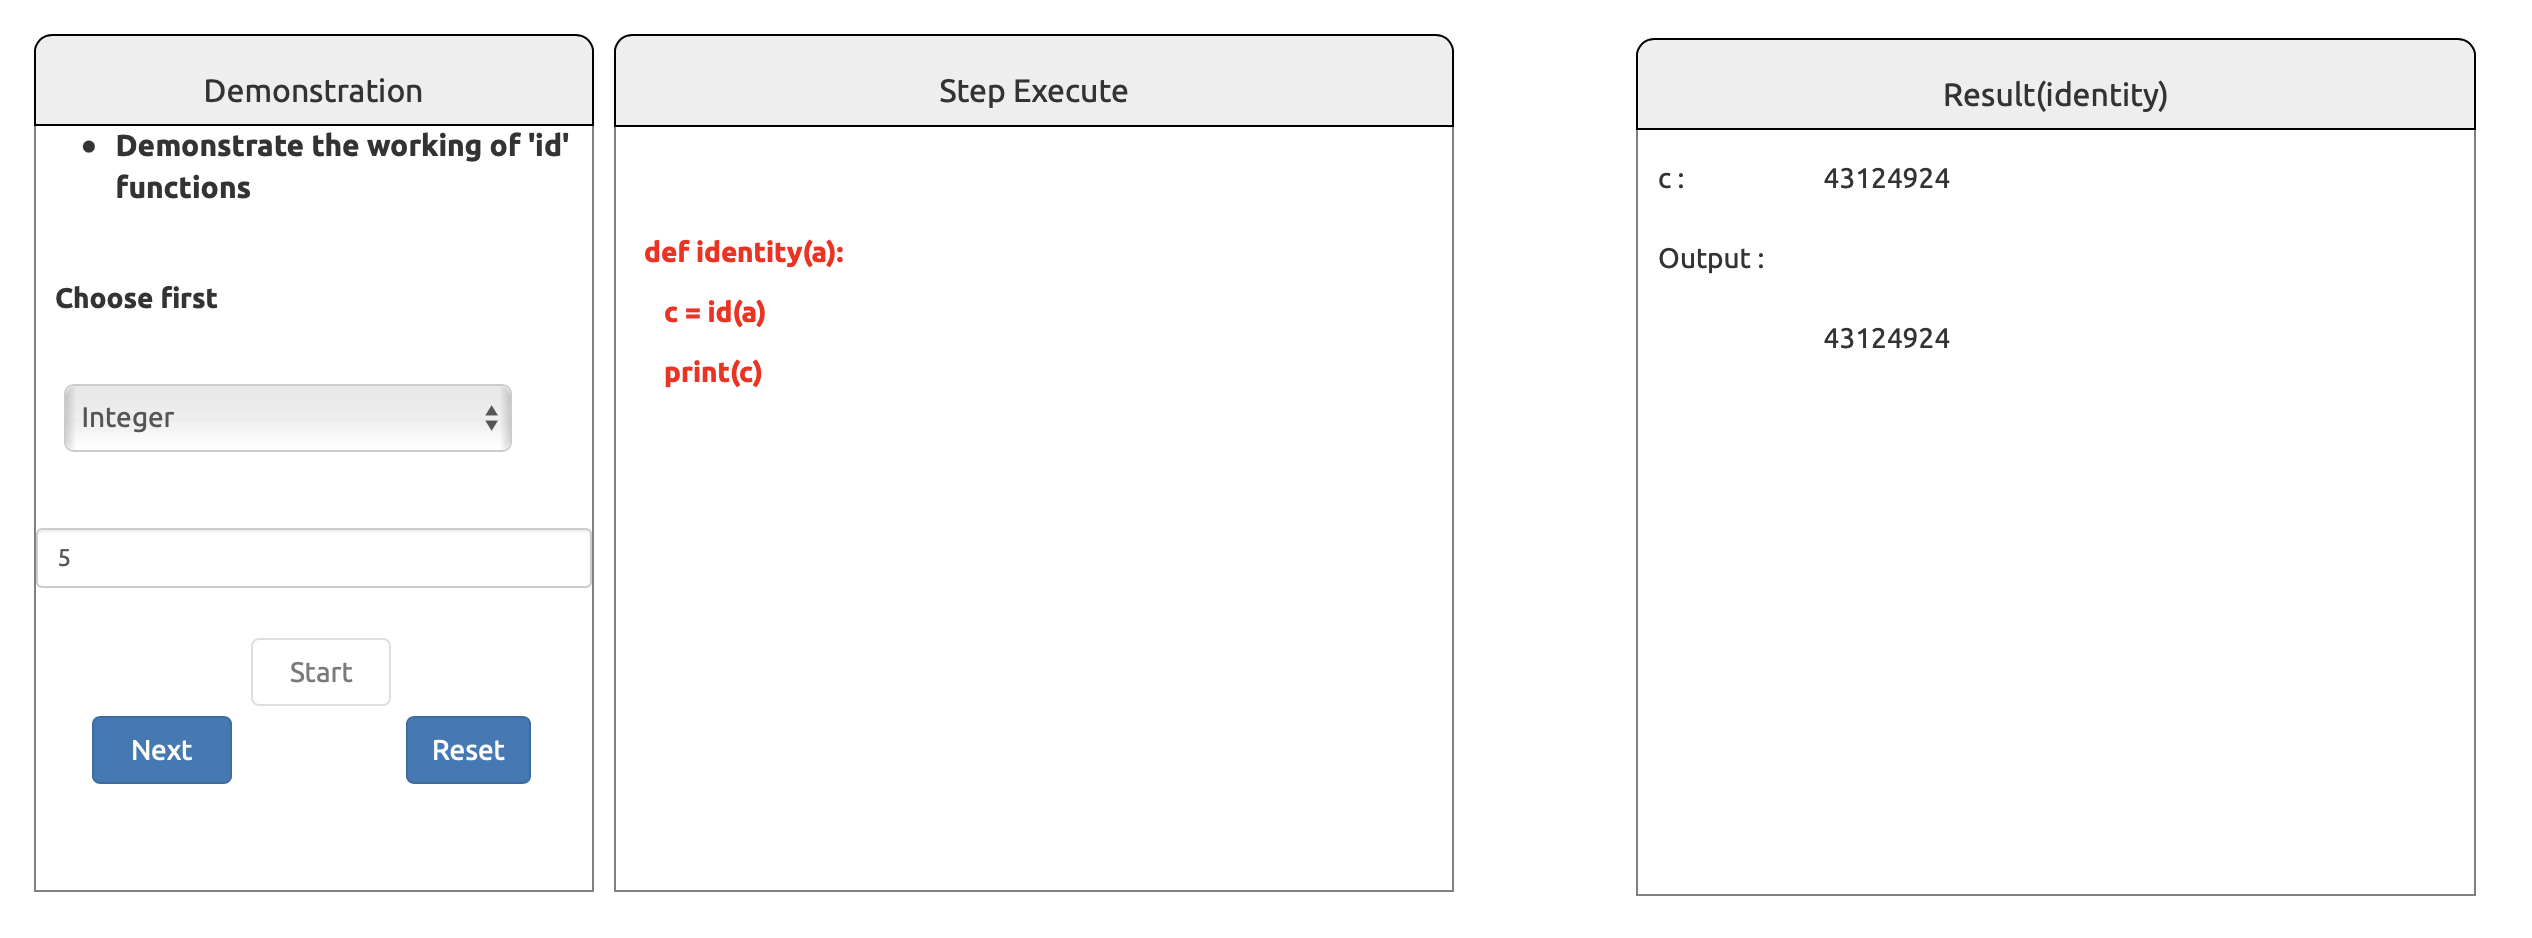
\includegraphics[width=0.8\linewidth]{images/existing-vlabs.png}
    \caption{The current implementation of virtual labs}
    \label{fig:existing-vlabs}
\end{figure}
\begin{figure}[h]
    \centering
    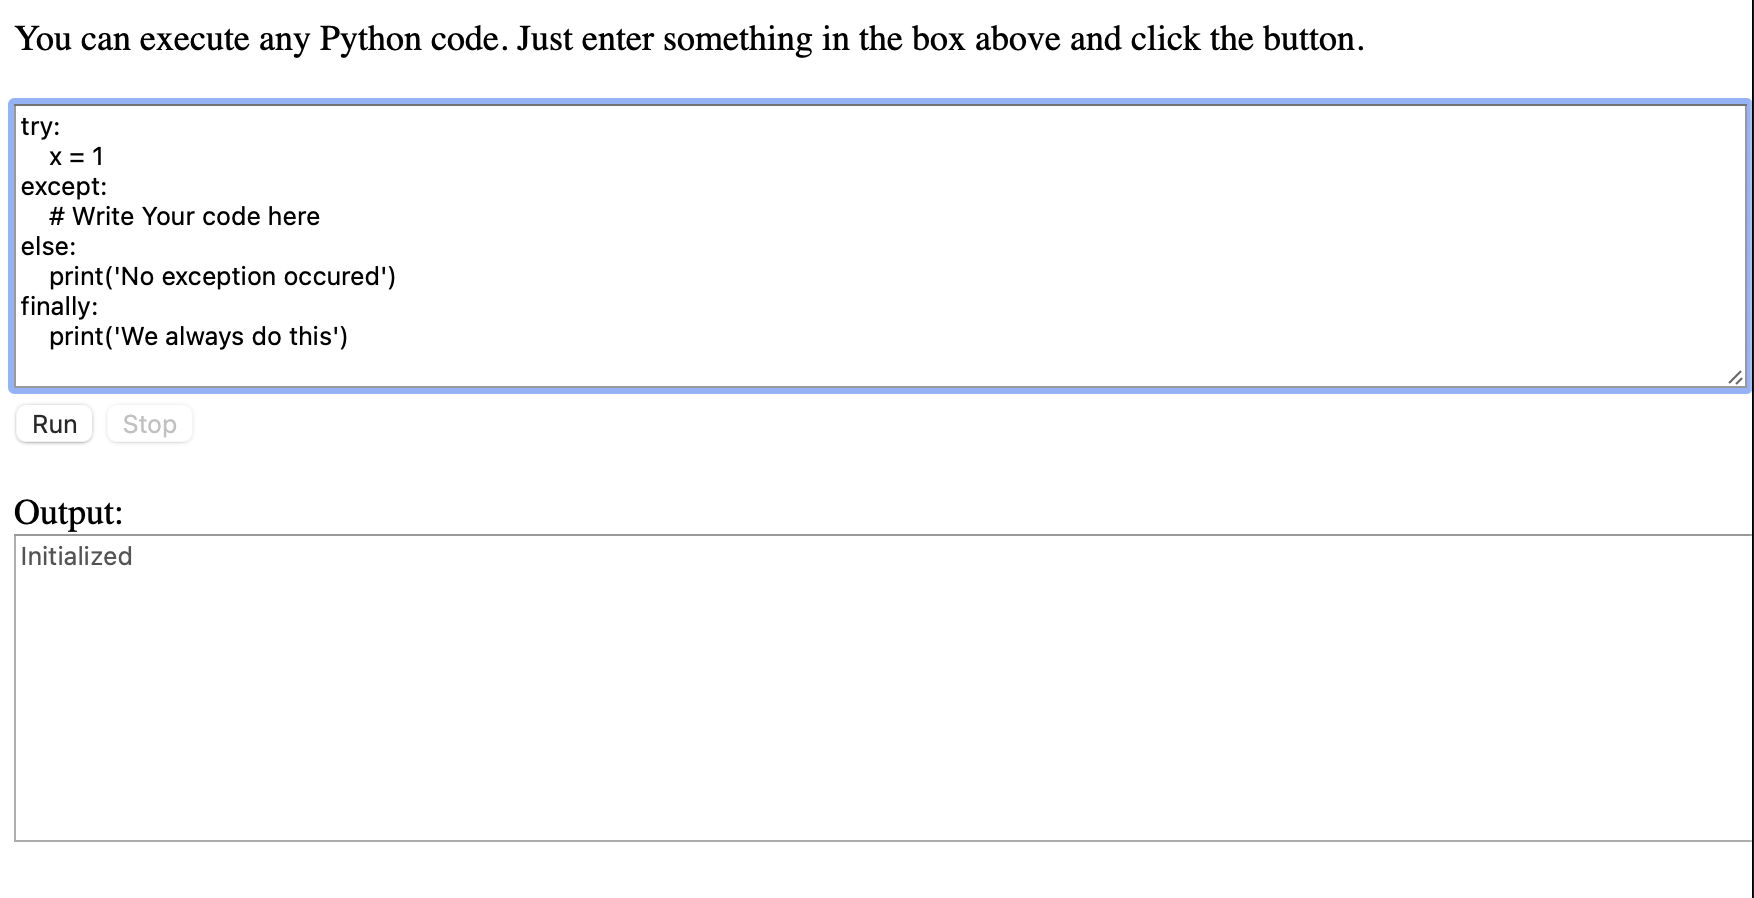
\includegraphics[width=0.8\textwidth]{images/impl-demo.png}
    \caption{Client side compiling using Pyodide}
    \label{fig:implementation}
\end{figure}
\\
For implementation, we closesly follow the documentation of Pyodide, and implement a very lightweight version of it. The screenshot of the same can be found in Fig \ref{fig:implementation}\footnote{Source code for the same can be found at \url{https://github.com/vjspranav/Pyodide-implementation}}. Considering all the requirements, we have a very basic implementation that takes care of:
\begin{itemize}
    \item Loading the python interpreter and running the code client side.
    \item Allowing a user to interrupt the execution of the code.
    \item Automatically stopping the execution of the code after a certain time limit.
    \item Disabling editing to a specific section of the code.
\end{itemize}


Intially we directly implemented using JS, and then from the bug analysis and requirement study we realised the requirement of code interrupt as discussed in 4.3. We go ahead with the implementation of the same using web workers.
The interruption is especially the focus as it can heavily influence the user's experience and can cause severe lags on the browser in cases of infinitiley running codes.

\section{Discussion}
Multiple online coding and education platforms like Virtual Labs, would need an exclusive backend server running if they intend on having code compilation. WebAssembly has brought in many new innovations, and if we could utilize it$’$s power to allow the compilation on browser itself it would save multiple such organisations a huge cost of having a backend server also at the same time, sideloading all the work to a client$’$s browser. We discuss how we come to a solution for each of the Research Questions that we had asked.

\subsection{RQ1: How will the implementation of a webassembly compiler help in the development of web applications?}
We do not have a strong ground to state a fixed answer here, but a very obvious positive impact would be the reduction in the cost of hosting a web application. The cost of hosting a web application is directly proportional to the number of users it has. If we could reduce the cost of hosting a web application, it would be a huge benefit for the organisation.\footnote{When we talk about cost of hosting a web application, we specifically are talking about the cost of hosting a backend server for compiling codes.} \\
This would also give an organisation power to use service worker and load these compilers without internet connection. This would allow the users to use the labs even when they are offline. \\
We discuss how we could add more validation to this in future work.

\subsection{RQ2: What are the challenges in implementing a webassembly compiler on client side?}
The only challenge that we face was the fact that multiple features such as threads, SIMD, and GC are not supported by browsers. This is a major challenge as these features are very important for a compiler to be able to compile a high level language.\\ 
Majority of these do not have any impact on our specific requirement which is geared towards a basic Python Programming Lab. \\

\subsection{RQ3: How big of an impact do bugs in WebAssembly compilers have on the implementation requirement of Virtual Labs?}
Although there are many bugs that exist in pyodide both resolved and unresolved, we see that the impact of these bugs is not very big on our implementation. We have been able to implement a basic Python Programming Lab with the help of pyodide. \\
The only issue that we had was to setup interrupts due to lack of support for signals webassembly. This as discussed was resolved using Web Workers which are not supported by all browsers widely. \\

\section{Conclusion}
In this paper we try to show the importance of having client side compilation. We conduct our study using Pyodide as a base, and answer the questions pertaining to bugs and implementation in a project. We realize the possibilities this brings to an organisation both interms of performarnce and resources required. \\
We also perform a bug analysis using a previously done research and validate the approaches and bugs from that paper. \\
We believe there is a huge scope by moving the compilation to the client side for all services that require a backend server for processing. This is because, even mobile devices are releasing with processors sufficient enough to run even AI models. This would greatly improve the lags caused by network latency and server loads and greatly improve the user experience. \\


%%
%% The acknowledgments section is defined using the "acks" environment
%% (and NOT an unnumbered section). This ensures the proper
%% identification of the section in the article metadata, and the
%% consistent spelling of the heading.
% \begin{acks}
% To Robert, for the bagels and explaining CMYK and color spaces.
% \end{acks}

%%
%% The next two lines define the bibliography style to be used, and
%% the bibliography file.
\bibliographystyle{ACM-Reference-Format}
\bibliography{base}

%%
%% If your work has an appendix, this is the place to put it.
\appendix
\input{sections/appendix/appendix1}

\end{document}
\endinput
%%
%% End of file `sample-authordraft.tex'.
